\chapter{Trusted and Optimized UAV Collision Avoidance}

\section{Collision Avoidance for Unmanned Aerial Vehicles} \label{sec:uavintro}

\begin{figure}
    \centering
    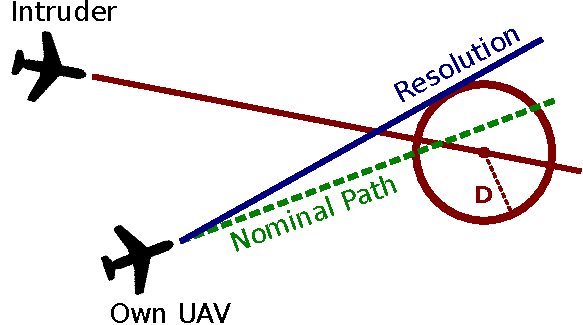
\includegraphics[height=5.0cm]{media/simple_trl.pdf}
    \caption[Trusted resolution logic]{Trusted resolution logic. The near mid air collision exclusion zone (circle with radius $D$) moves with the intruder through time, but is shown here only at the time of closest approach. The TRL (\Cref{alg:trl}) finds a straight trajectory close to the nominal path that avoids this zone.}
    \label{fig:trl}
\end{figure}

As unmanned aerial vehicles (UAVs) move toward full autonomy, it is vital that they be capable of effectively responding to anomalous events, such as the intrusion of another aircraft into the vehicle's flight path. Minimizing collision risk for aircraft in general, and UAVs in particular, is challenging for a number of reasons. First, avoiding collision requires planning in a way that accounts for the large degree of uncertainty in the future paths of the aircraft. Second, the planning process must balance the competing goals of ensuring safety and avoiding disruption of normal operations. Many approaches have been proposed to address these challenges \cite{JKK-LCY:00,HYO-MJK:15,RB-CF-HE:09,GH-RB-JM:11,HH-JJ-CM:10,AN-CM-GD:12,ST-MJK-LPK-TLP-JKK:10,MJK-JPC:11,MJK-JPC-LPK-TL:10,LPK-TL:09,HB-DH-MJK-WSL:12,JEH-MJK-WAO:13,EJR:14}.

At present, there are two fundamentally different approaches to designing a conflict resolution system.The first approach focuses on inspiring confidence and trust in the system by making it as simple as possible for government regulators and vehicle operators to understand.
This is accomplished by constructing the algorithm using hand-specified rules.
Several algorithms that fit this paradigm have been proposed, and research toward formally verifying their safety-critical properties is underway \cite{RB-CF-HE:09,GH-RB-JM:11,HH-JJ-CM:10,AN-CM-GD:12}.  In this chapter, I will  refer to such algorithms as \emph{trusted resolution logic} (TRL).
Many TRL systems have a number of parameters that determine how conservatively the system behaves.
These parameters may be tuned to meet specific performance goals, but their exact affects on performance can typically only be characterized empirically.

The second approach focuses on optimizing performance.
This entails the offline or online  computation of a ``best" response action. Dynamic programming is widely used for this task \cite{ST-MJK-LPK-TLP-JKK:10,MJK-JPC:11,MJK-JPC-LPK-TL:10,LPK-TL:09,HB-DH-MJK-WSL:12,JEH-MJK-WAO:13}. 
Conflict resolution systems designed using this approach will be referred to as \emph{directly optimized} systems. 
Unfortunately, even if a conflict resolution system performs well in simulation, government regulators and vehicle operators will often (and sometimes rightly) be wary of trusting its safety due to perceived complexity and unpredictability.
Even in the best case, such a system would require expensive and time-consuming development of tools for validation as was the case for the recently developed replacement for the traffic alert and collision avoidance system (TCAS) \cite{JEH-MJK-WAO:13}. 

This chapter proposes two conflict resolution strategies that combine the strengths of trusted resolution logic and direct optimization approaches.
In both strategies, dynamic programming is used to find near-optimal actions for each state.
The difference lies in the set of actions available to the optimizer.
In the \emph{optimized TRL} approach, the actions are a set of certified TRL parameters.
In the \emph{trusted direct optimization} approach, the actions are a state-dependent set of immediate response actions that are deemed safe by certified TRL.
Both strategies may achieve better performance than the base TRL with a similar relative ease of certification compared to plain direct optimization.

We test the new approaches in a scenario containing a UAV equipped with a perfect (noiseless) sensor to detect the state of an intruder and a simple reference TRL to resolve conflicts. This TRL, illustrated in \Cref{fig:trl}, determines a path that does not pass within a specified separation distance, $D$, of the intruder given that the intruder maintains its current heading (except in cases where no such path exists or when the TRL's heading resolution is too coarse to find such a path).
This reference TRL is described in more detail in \Cref{sec:trl}.

To account for uncertainty in the intruder's flight path, if $D$ takes a constant value, say $\bar{D}$, the value must be very large to ensure safety, but this may cause unnecessary departures from normal operation.
To overcome this limitation and ensure safety without being too conservative, I apply implementations of the two strategies outlined above.
The optimized TRL approach computes a policy, $\trl{\pi}$, that specifies a time varying separation distance, $D_t$, for each encounter state, while the direct optimization and trusted direct optimization approaches compute policies, $\diro{\pi}$ and $\tdo{\pi}$, that specifies a bank angle, $\phi_t$ for each encounter state.
For this reason, symbols referring to the optimized TRL approach generally have subscript $D$, while those referring to direct optimization trusted direct optimization have a subscript $\phi$.

The problem of dynamically selecting actions $D_t$ or $\phi_t$ can be formulated as a Markov decision process (MDP). Online solution of $\trl{\pi}$, $\diro{\pi}$, or $\tdo{\pi}$ using an algorithm such as Monte Carlo Tree Search (MCTS) \cite{AC-JH-NS-OT-NB:11} would be conceptually straightforward, but would require significant computing power onboard the vehicle, and it would be difficult and time-consuming to rigorously certify the implementation of MCTS due to its reliance on pseudo-random number generation. A key contribution of this chapter is to devise an \emph{offline} approach to compute the policies. Offline optimization is difficult because of the size of the state space of the MDP, which is the Cartesian product of the continuous state spaces of the UAV and the intruder. To overcome this challenge, I devise a value function approximation scheme that uses grid-based features that exploit the structure of the state space. This value function is optimized using simulation-based approximate dynamic programming. The policy is then encoded using an approximate post-decision state value function. Armed with this post-decision value function, the UAV can easily extract the optimal action for the current state online by evaluating each possible action.


\section{MDP Models}\label{sec:uavmodel}

The problem of avoiding an intruder using one of the strategies above is formulated as an MDP, referred to as an \emph{encounter} MDP. An encounter involves two aerial vehicles flying in proximity. The first is the vehicle for which the resolution controller is being designed, which will be referred as the ``own UAV" (or simply ``UAV''). The second is the intruder vehicle, which may be manned or unmanned and will be referred to as the ``intruder". Specifically, the encounter MDP is defined by the tuple $(\sspace, \aspace, \tdist, R)$, which consists of

\begin{itemize}
    \item The state space, $S$: The state of the encounter, $s$, consists of (1) the state of the own UAV, $\rs$, (2) the state of the intruder, $\is$, and (3) a boolean variable $\dev$. The variable $\dev$ is set to true if the UAV has deviated  from its nominal course. Collectively, the state is given by the triple
        \begin{equation}
            s = \left(\rs, \is, \dev\right) \text{.}
        \end{equation}
        The state components $\rs$ and $\is$ are specified in Section \ref{sec:veh}.
        To model termination, the state space $S$ includes a ``dummy" termination state, denoted with $\sterm$.
    \item The action space, $A$: The action space differs for the two approaches as described in detail in \Cref{sec:aspaces}. $a$ will be used to refer to all types of action depending on the context.
    \item The state transition probability density function, $T: S \times A \times S \to \mathbb{R}$: The value $T(s,D,s')$ is the probability density of transitioning to state $s'$ given that the separation parameter $D$ is used within the TRL at state $s$. This function is implicitly defined by a generative model that consists of a state transition function $F(\cdot)$ (described in \Cref{sec:control}) and a stochastic process $W$ (described in \Cref{sec:veh}).
    \item The reward, $\reward:\sspace \times \aspace \to \reals$: The reward function, defined in \Cref{sec:rew}, rewards reaching a goal and penalizes near mid air collisions (NMACs), deviation from the nominal path, and time outside a goal region.
\end{itemize}

\subsection{Model Assumptions}\label{sec:assumptions}

% SHORTEN: this could be more concise
Two important simplifying assumptions were made for this initial study. First, the UAV and the intruder move only in the horizontal plane and at constant speed. Modeling horizontal maneuvers is necessary because UAVs will likely have to employ horizontal maneuvers in place of or in addition to the vertical maneuvers that current collision avoidance systems for manned aircraft such as TCAS rely on. This is due to both climb performance limitations and regulatory constraints such as the \num{400}\si{ft} ceiling for small (\num{<55}\si{lb}) commercial UAVs in Federal Aviation Administration rules \cite{faa2018small}. Constraining altitude and speed simplifies exposition and reduces the size of the state space, keeping the computational burden modest compared with a formulation that includes variable altitude and speed. Extensions to higher fidelity models (e.g.,~\cite{MJK-MWME-LPE-JKK-JDG:10}) are possible and left for future research.
A higher fidelity model would present a computational challenge, but perhaps not an insurmountable one.
For example, the TRL could be extended to handle variable speed and altitude, but the policy could be optimized only on the most important dimensions of the model (e.g., the horizontal plane). See~\cite{MJK-JPC-PPR:10} for a similar successful example.

Second, the intruder dynamics are \emph{independent} of the UAV's state; in other words, the intruder does not react to the flight path of the UAV. The cooperative setting where both the UAV and the intruder are equipped with a collision avoidance system (CAS) \cite{EJR:14,CT-GJP-SSS:98,MJK-JPC:11} is left for future research.

\subsection{Vehicle States and Dynamics}\label{sec:veh}

This paper uses a very simple discrete-time model of an encounter between two aerial vehicles with time steps of duration $\Delta t$. Throughout this section, the superscripts $\own{}$ and $\intr{}$ refer to the own UAV and intruder quantities, respectively, while the superscript $\either{}$ may be replaced by either $\own{}$ or $\intr{}$. Both the UAV's and the intruder's states consist of the horizontal position $(x,y)$ and heading $\psi$, that is
\begin{equation}
    \rs = \left(\own{x}, \own{y}, \own{\psi} \right)\text{,} \quad 
    \is = \left(\intr{x}, \intr{y}, \intr{\psi} \right)\text{.}
\end{equation}
The UAV and intruder also have similar dynamics. Both aircraft fly forward in the horizontal plane at constant speeds denoted by $\either{v}$. They may turn at rates $\either{\dot{\psi}}$ that remain constant over the simulation step. The following equations define the vehicle dynamics: 
\begin{align*}
    \either{x}_{t+1} &= \begin{cases}
        \either{x}_{t} + \either{v} \cos\left(\either{\psi}_t\right)\Delta t & \text{if } \either{\dot{\psi}} = 0 \\
        \either{x}_{t} + \either{v} \frac{\sin\left( \either{\psi}_t + w_t\Delta t \right) - \sin\left( \either{\psi}_t \right)}{\either{\dot{\psi}}} & \text{otherwise}\\
    \end{cases} \\
    \either{y}_{t+1} &= \begin{cases}
        \either{y}_{t} + \either{v} \sin\left(\either{\psi}_t\right)\Delta t & \text{if } \either{\dot{\psi}} = 0 \\
        \either{y}_{t} - \either{v} \frac{\cos\left(\either{\psi}_t + \either{\dot{\psi}}\Delta t\right) - \cos\left(\either{\psi}_t\right)}{\either{\dot{\psi}}} & \text{otherwise}\\
    \end{cases} \\
    \either{\psi}_{t+1} &= \either{\psi}_t + \either{\dot{\psi}} \Delta t \text{.}
\end{align*}

The intruder makes small random turns with
\begin{equation}
    \intr{\dot{\psi}} = w_t \text{,}
\end{equation}
where $w_t$ is a stochastic disturbance. We let $W$ denote the stochastic process $\{w_t: t\in \naturals\}$. The random variables $w_t$ in $W$ are assumed independent and identically normally distributed with zero mean and a specified standard deviation, $\sigma_{\dot{\psi}}$. Subsequently, the intruder dynamics will be collectively referred to as $\intr{f}$, and
\begin{equation} \label{eq:idyn}
    \intr{s_{t+1}} = \intr{f}\left(\intr{s}_t, w_t\right) \text{.}
\end{equation}


The dynamics of the  UAV are simplified conventional fixed wing aircraft dynamics with a single input, namely the roll angle $\own{\phi}$. We assume that the roll dynamics are  fast compared to the other system dynamics, so that the roll angle $\own{\phi}$  may be directly and instantaneously commanded by the control system. This assumption avoids the inclusion of roll dynamics, which would increase the size of the state space.
\begin{equation}
    \own{\dot{\psi}_t} = \frac{g \tan \own{\phi}_t}{\own{v}} \text{,}
\end{equation}
where $g$ is acceleration due to gravity. The performance of the UAV is limited by a maximum bank angle
\begin{eqnarray}
    |\own{\phi}_t| \leq \phi_\text{max} \text{.}
\end{eqnarray}
The UAV dynamics will be collectively referred to as $\own{f}$, and
\begin{equation} \label{eq:odyn}
    \own{s_{t+1}} = \own{f}\left(\own{s}_t, \own{\phi}_t\right) \text{.}
\end{equation}

\subsection{Transition Function} \label{sec:control}

It will often be convenient to refer to all of the dynamics in the state transition with a single transition function, which will be defined below after defining additional behavior regarding goals and near mid-air collisions.

The goal region that the UAV is trying to reach is denoted by $S_\text{goal}$. This is the set of all states in $S$ for which $\left\|\left(\own{x}, \own{y}\right) - \left(\own{x}_{\text{goal}}, \own{y}_{\text{goal}}\right)\right\| \leq \dgoal$, where $\dgoal>0$ is a specified goal region radius, and $\left(\own{x}_{\text{goal}}, \own{y}_{\text{goal}}\right)$ is the goal center location.
A near mid air collision (NMAC) occurs at time $t$ if the UAV and intruder are within a minimum separation distance, $\dnmac > 0$, that is if $\left\|\left(\own{x}_t, \own{y}_t\right) - \left(\intr{x}_t, \intr{y}_t\right)\right\| \leq \dnmac$.
If the UAV reaches the goal region at some time $t$, i.e., $s_t \in S_\text{goal}$, or if an NMAC occurs, the overall encounter state $s$  transitions to the terminal state $\sterm$ and remains there.  If the UAV performs a turn, $\dev$ is set to true because the vehicle has now deviated from the nominal straight path to the goal.

Let the state transition function, defined by \eqref{eq:idyn}, \eqref{eq:odyn}, and the special cases above, be denoted concisely as $F$ so that  
\begin{equation}\label{eq:sys_dyn}
    s_{t+1} = F(s_t, \own{\phi}_t, w_t) \text{,}
\end{equation}


\subsection{Reference Trusted Resolution Logic}\label{sec:trl}

The numerical tests use the simple reference TRL shown in \cref{fig:trl}.
The TRL determines a heading angle, $\psires$, that is close to the heading to the goal, $\psigoal$, and that will avoid future conflicts with the intruder given that the intruder maintains its current heading. This is shown in Figure~\ref{fig:trl}.

\subsubsection{Minimum Separation Distance}

Given an initial state $s$, a candidate heading for the UAV, $\psicand$, and that both vehicles maintain their heading, the distance between the vehicles at the time of closest approach is a simple analytical function. Specifically, consider the distance  $d\left(s,\psicand,\tau\right)$ between the vehicles $\tau$ time units in the future, i.e., 
\begin{equation} \label{eqn:dist}
    d\left(s, \psicand, \tau\right) = \sqrt{\Delta x(\tau)^2 + \Delta y(\tau)^2} \text{,}
\end{equation}
where
\begin{align*}
    \Delta x(\tau) &= \intr{x} - \own{x} + \tau \intr{v} \cos\left(\intr{\psi}\right) - \tau \own{v} \cos\left(\psicand\right),\\
    \Delta y(\tau) &= \intr{y} - \own{y} + \tau \intr{v} \sin\left(\intr{\psi}\right) - \tau \own{v} \sin\left(\psicand\right) \text{.}
\end{align*}

The minimum distance between the two vehicles is analytically found by setting the time derivative of $d\left(s,\psicand, \tau\right)$ to zero. Specifically, the time at which the vehicles are closest is given by
\begin{equation}
    \tau_\text{min}\left(s,\psicand\right) = \max \left\{\frac{a + b}{c-2d}, 0\right\} \text{,}
\end{equation}
where
\begin{align*}
    a &:= -\intr{v}\intr{x} \cos(\intr{\psi}) - \intr{v} \intr{y} \sin(\intr{\psi}) \\
    b &:= \own{v} \intr{x} \cos(\psicand) + \own{v} \intr{y} \sin(\psicand) \\
    c &:= v^{(\ownid)\,2} + v^{(\intrid)\,2}\cos^2(\intr{\psi}) + v^{(\intrid)\,2}\sin^2(\intr{\psi}) \\
    d &:= \own{v}\intr{v} ( \cos(\intr{\psi})\cos(\psicand) + \sin(\intr{\psi})\sin(\psicand) ) \text{.}
\end{align*}
The minimum separation distance over all future time is then
\begin{equation}
    d_\text{min}\left(s, \psicand\right) := d\left(s, \psicand, \tau_\text{min}\left(s,\psicand\right)\right) \text{.}
\end{equation}

It will also be occasionally convenient to use $d_\text{min}$ with only a state as an argument.
In this case, $\psicand$ should be understood to be the UAV heading angle corresponding to that state, that is $d_\text{min}(s) := d_\text{min}(s, \own{\psi})$ where $\own{\psi}$ is the UAV heading in $s$.

\subsubsection{Discrete Heading Optimization}

The TRL begins with a discrete set of potential heading values (each denoted $\psicand$) for the UAV. It then determines, for a desired separation distance $D$,  which of those will not result in a collision given that the UAV and  intruder maintain their headings. Finally, it selects the value from that set which is closest to $\psigoal$. The TRL is outlined in \cref{alg:trl}.

\renewcommand{\algorithmicrequire}{\textbf{Input:}}
\renewcommand{\algorithmicensure}{\textbf{Output:}}
\begin{algorithm}[tb]
    \caption{Trusted Resolution Logic}\label{alg:trl}
\begin{algorithmic}
    \Require Encounter state $s$, desired separation distance $D$
    \Ensure Resolution heading angle $\psires$
        \Function{$\text{TRL}$}{$s$, $D$}
        \State $\Psi \gets \left\{\own{\psi} + n\pi/N : n \in \{-N,\ldots,N\} \right\}$
        \Comment{range of values for heading}
        \State $D^* = \underset{\psicand \in \Psi}{\max}\, d_\text{min}\left(s, \psicand\right)$
        \If{$D^*< D$} \Comment{conflict inescapable}
            \State $\Psi \gets \left\{\psicand \in \Psi : d_\text{min}\left(s, \psicand\right) = D^*\right\}$
            \State \Return $\underset{\psicand \in \Psi}{\argmin}\,|\psicand-\psigoal|$
        \Else
            \State $\Psi \gets \left\{\psicand \in \Psi : d_\text{min}\left(s, \psicand\right) \geq D\right\}$
            \State \Return $\underset{\psicand \in \Psi}{\argmin}\,|\psicand-\psigoal|$
        \EndIf
    \EndFunction
\end{algorithmic}
\end{algorithm}


\subsection{Action Spaces and Control Systems}\label{sec:aspaces}

The numerical experiments consider policies generated by solving three different MDPs, each with a different action space. 
For the sake of conciseness, $a$ will be used to represent any type of action depending on the context.

\subsubsection{Direct Optimization}

In the direct optimization approach, the actions are simply the bank angles less than $\phi_\text{max}$, that is $\diro{\aspace} = \left\{\phi \in \reals: |\phi| \leq \phi_\text{max} \right\}$.

\subsubsection{Trusted Direct Optimization}

In the trusted direct optimization approach, the set of actions is state dependent.
Specifically, it is the set of bank angles that the TRL deems safe, that is $\tdo{\aspace}(s) = \left\{\phi \in \diro{\aspace}: d_\text{min}(F(s, \phi, 0)) > D_\text{NMAC} \right\}$.

\subsubsection{Optimized TRL}

In the optimized TRL approach, the actions are the possible values for the separation distance, that is $\trl{\aspace} = D\in \reals_{\geq 0}$ used in the TRL (see Figure \ref{fig:trl}).
A simple low level control system converts the desired heading from the TRL (denoted $\psires$) and into a bank angle for the vehicle.
We write this as
\begin{equation}
    \own{\phi}_t = c\left(\own{s}_t, \psires \right) \text{,}
\end{equation}
where $c(\cdot)$ represents the low level controller.
When the action is a separation distance, the transition function, $F$, should be understood to contain the TRL and low level control system, that is
\begin{equation}
    F(s_t, D_t, w_t) := F(s_t, c(\own{s}_t, \text{TRL}(s_t, D_t), w_t) \text{.}
\end{equation}

\subsection{Reward}\label{sec:rew}

This section considers optimization of two competing metrics. The first goal is to minimize the risk of a NMAC. This aspect of performance is quantified with the fraction of NMACs prevented. The second goal is to minimize the probability of deviation from the nominal path. This metric was chosen (as opposed to a metric that penalizes the size of the deviation) because, in a commercial setting, any deviation from the normal operating plan might have a large cost in the form of disrupting schedules, preventing a mission from being completed, or requiring manual human monitoring. The MDP reward function is designed to encourage the policy towards a solution that performs well with respect to these goals.  

Specifically, the utility associated with an encounter is the sum of the stage-wise rewards throughout  the entire encounter
\begin{equation}\label{eqn:encrew}
    \sum_{t=0}^\infty R(s_t, a_t) \text{.}
\end{equation}

In order to meet both goals, the stage-wise reward is
\begin{align}\label{eqn:rew}
    \reward(s_t, a_t) := & - c_\text{step} + r_\text{goal} \times \operatorname{in\_goal}\left(\own{s}_t\right) \nonumber\\
             & - c_\text{dev} \times \operatorname{causes\_deviation}(s_t, a_t) \nonumber\\
             & - \lambda \times \operatorname{is\_NMAC}(s_t) \text{,}
\end{align}
for positive constants $c_\text{step}$, $r_\text{goal}$, $c_\text{dev}$,  and $ \lambda$. The first term is a small constant cost accumulated in each step to push the policy to quickly reach the goal. The function $\operatorname{in\_goal}$ indicates that the UAV is within the goal region, so the second term is a reward for reaching the goal. The third term is a penalty for deviating from the nominal path. The function $\operatorname{causes\_deviation}$ returns $1$ if the action will cause a deviation from the nominal course and $0$ otherwise. It will only return $1$ if the vehicle has not previously deviated and $\dev$ is false, so the penalty may only occur once during an encounter. This behavior makes the inclusion of $\dev$ in the state necessary. Constants $c_\text{step}$, $r_\text{goal}$, and $c_\text{dev} $ represent relative weightings for the terms that incentivize a policy that reaches the goal quickly and minimizes the probability of deviation. Example values for these constants  are given in \Cref{sec:results}. The fourth term is the cost for a collision. The weight $\lambda$ balances the two performance goals. We heuristically expect there to be a value of $\lambda$ for which the solution to the MDP meets the desired risk ratio if it is attainable. Bisection, or even a simple sweep of values can be used to find a suitable value, and this method has been used previously to analyze the performance of aircraft collision avoidance systems \cite{HB-DH-MJK-WSL:12,MJK-JPC:11}.

\subsection{Problem statement}
The problem we consider  is to find a feedback control policy $\pi^*: S \to A$, mapping an encounter state $s_t$ into an action $a_t$,  that maximizes the expected reward \eqref{eqn:encrew} subject to the system dynamics \eqref{eq:sys_dyn}:
\begin{equation}\label{eq:prob}
\begin{aligned}
& \underset{\pi}{\text{maximize}}
& & E \left[\sum_{t=0}^\infty R(s_t, \pi(s_t))\right] \\
& \text{subject to}
& & s_{t+1} = F(s_t, \pi(s_t), w_t) \text{,}
\end{aligned}
\end{equation}
for all initial states $s_0 \in S$. To make the solution of problem \eqref{eq:prob} practical, we present an approximate dynamic programming approach that yields a suboptimal policy, $\tilde{\pi}$, in the next section.

\section{Solution Approach} \label{sec:approach}

Since the problem \eqref{eq:prob} has continuous state and action spaces and complex dynamics, it is difficult to solve.
In order to make it more tractable, two approximations are used.

First, only a small number of discrete actions, which will be referred to as $\tilde{\aspace}$, are considered. Specifically, for the optimized TRL, direct optimization, and trusted direct optimization approaches, the following action spaces are used:
\begin{align}
    \trl{\tilde{\aspace}} &= \{\dnmac, \allowbreak 1.5 \dnmac, \allowbreak 2 \dnmac, \allowbreak 3 \dnmac, \allowbreak 4 \dnmac \} \\
    \diro{\tilde{\aspace}} &= \left\{-\phi_\text{max},-\frac{\phi_\text{max}}{2}, 0, \frac{\phi_\text{max}}{2},\phi_\text{max}\right\} \\
    \tdo{\tilde{\aspace}}(s) &= \left\{\phi \in \diro{\tilde{\aspace}} : d_\text{min}\left(F(s, \phi, 0)\right) > D_\text{NMAC} \right\} \text{.}
\end{align}

The second approximation is the approximate value iteration algorithm \cite{DB:05} used to optimize the policy. The value function, $V$, represents the expected value of the future reward given that the encounter is in state $s$ and an optimal policy will be executed in the future. We approximate $V$ with a linear architecture of the form  \cite{DB:05}
\begin{equation}\label{eqn:val}
    \tilde{V}(s) = \beta(s)^\top \theta \text{,}
\end{equation}
where the feature function $\beta$ returns a vector of $N_\beta$ feature values, and $\theta\in \reals^{N_\beta}$ is a vector of weights \cite{DB:05}. At each step of  value iteration, the weight vector $\theta$ is fitted to the results of a large number of single-step simulations by solving a linear least-squares problem. After value iteration has converged, $\tilde{V}$ is used to estimate a \emph{post-decision state} value function, $\tilde{V}_q$,  which is also approximated using a linear combination of features. The policy is extracted online in real time by selecting the action that results in the post-decision state that has the highest value according to $\tilde{V}_q$. The choice of working with post-decision states will be discussed in \Cref{sec:extract}.

\subsection{Approximate Value Iteration} \label{sec:iter}

The bulk of the computation is carried out offline before vehicle deployment using simulation. Specifically, the first step is to estimate the optimal value function for problem \eqref{eq:prob} using value iteration \cite{DB:05}. On a continuous state space such as the encounter state space used in this work, the Bellman operator used in value iteration cannot be applied for each of the uncountably infinite number of states, so an approximation must be used. In this paper we adopt projected value iteration \cite{DB:05}, which  uses a finite number of parameters to approximate the value function. Each successive approximation, $\tilde{V}_k$, is the result of the Bellman operation projected onto a linear subspace with respect to the Euclidean norm, that is
\begin{equation}\label{eqn:projvi}
    \tilde{V}_{k+1}(s) = \Pi \mathcal{B}[\tilde{V}_k](s) \text{,}
\end{equation}
where $\mathcal{B}$ is the Bellman operator, and $\Pi$ is a projection onto the linear subspace $\Phi$ spanned by the $N_\beta$ basis functions (see \cite{DB:05} for a detailed discussion of this approach).

To perform the approximate value iteration \eqref{eqn:projvi}, we resort to Monte Carlo simulations. Specifically, for each iteration, $N_\text{state}$ states are uniformly randomly selected. If the states lie within the grids used in the feature function (see \Cref{sec:features}) the sample is ``snapped'' to the nearest grid point to prevent approximation errors due to the Gibbs phenomenon \cite{JF-FBR:91}. At each sampled state $s^{[n]}$, $n=1,\ldots, N_\text{state}$, the stage-wise reward and the expected value of the value function are evaluated for each action $a$ in $\tilde{\aspace}$. The expectation embedded in the Bellman operator is approximated using $N_{\text{EV}}$ \emph{single-step} intruder simulations, each with a randomly generated noise value, $w_m$, $m=1,\ldots, N_{\text{EV}}$. However, since the own UAV dynamics are deterministic, only one own UAV simulation is needed. The maximum over $\tilde{A}$ is selected and stored as the $n$th entry of a vector $v_{k+1}$:
\begin{equation}
    v_{k+1}[n] := \max_{a \in \tilde{A}} \left\{R(s^{[n]},a) + \frac{1}{N_{\text{EV}}}\sum_{m=1}^{N_{\text{EV}}} \beta(F(s^{[n]}, a, w_m))^\top \theta_k \right\} \text{,}
\end{equation}
for $n=1,\ldots, N_\text{state}$. Here $v_{k+1}$ provides an approximation to the (unprojected) value function. To project $v_{k+1}$ onto $\Phi$, we compute the weight vector $\theta_{k+1}$ by solving the least-squares optimization problem
\begin{equation}
    \theta_{k+1} = \underset{\theta\in \reals^{N_\beta}}{\argmin} \sum_{n=1}^{N_\text{state}} \left( \beta\left(s^{[n]}\right)^\top \theta - v_{k+1}[n] \right) ^2 \text{.}
\end{equation}
Iteration is terminated after a fixed number of steps, $N_{VI}$, and the resulting weight vector, denoted by $\theta$, is stored for the next processing step (Section \ref{sec:extract}).

\subsection{Post Decision Value Function Extraction} \label{sec:extract}

For reasons discussed in \Cref{sec:policy}, our second step is to approximate a value function defined over post-decision states \cite{DB:05}. A post-decision state, denoted by $q$, is defined as a state in $S$ consisting of the own UAV state and $\dev$ \emph{at one time step into the future} and the intruder state \emph{at the current time}, that is
\begin{equation} \label{eqn:pd}
    q_t = \left(\rs_{t+1}, \is_t, \dev_{t+1}\right) \text{.}
\end{equation}
Correspondingly, let $g:S\times A\to S$ be the function that maps the current state and action to the post-decision state. In other words, function $g(s_t,a_t)$ returns $q_t$ consisting of
\begin{align}\label{eqn:g}
    \rs_{t+1} &= \own{f}\left(\rs_t, a_t \right) \nonumber\\
    \is_t     &= \is_t \nonumber\\
    \dev_{t+1} &= \max\{\dev, \text{causes\_deviation}(s_t,a_t)\} \text{.}
\end{align}

The approximate value function over post-decision states, $\tilde{V}_q$, is computed as follows.
Let $h:S \times \reals \to S$ be a function that returns the next encounter state given the post decision state and intruder heading noise value, that is $h(q_t,w_t)$ returns $s_{t+1}$ consisting of
\begin{align}
    \own{s}_{t+1} &= \own{s}_{t+1} \\
    \intr{s}_{t+1} &= \intr{f}(\intr{s}_{t}, w_t) \\
    \dev_{t+1} &= \dev_{t+1} \text{,}
\end{align}
where $\left(\own{s}_{t+1}, \intr{s}_t, \dev_{t+1}\right)$ are the members of $q_t$.

The value function $\tilde{V}_q$ can then be expressed in terms of $\tilde{V}$ as
\begin{equation} \label{eqn:pdest}
    % V_q(q) = \underset{s'}{E} \left[ V(s') | q \right] ,
    \tilde{V}_q(q) = \underset{w_t}{E} \left[ \tilde{V}\left(h\left(q,w_t\right)\right) \right] \text{,}
    % not sure whether this notation is correct at all
\end{equation}
where $w_t$ denotes, as usual, a random variable with Gaussian normal density.  Equation \eqref{eqn:pdest} implies that $\tilde{V}_q$ can also be approximated according to a linear architecture 
\begin{equation}
    \tilde{V}_q(q) = \beta(q)^\top \theta^q \text{,}
\end{equation}
where $\beta(q)$ is the  feature vector for post-decision states $q\in S$, and $\theta^q \in \reals^{N_\beta}$ is the corresponding weight vector.


Specifically, $N_q$ post decision states are randomly selected using the same method as described in \Cref{sec:iter} and are denoted as $q^{[n]}$, $n=1,\ldots, N_q$. For each sampled state $q^{[n]}$, the expectation in (\ref{eqn:pdest}) is approximated using $N_{\text{EV}}$ single-step simulations. The results are used to solve a least squares optimization problem
\begin{equation}
    \theta^q = \underset{\theta \in \reals^{N_{\beta}}}{\argmin} \sum_{n=1}^{N_q} \left( \beta \left(q^{[n]}\right)^\top \theta - v^q[n]\right) ^2 \text{,}
\end{equation}
where
\begin{equation}
    v^q[n] := \frac{1}{N_{\text{EV}}} \sum_{m=1}^{N_{\text{EV}}} \beta\left(h\left(q^{[n]},w_m\right)\right)^\top \theta \text{,}
\end{equation}
where $w_m$, $m=1,\dots,N_\text{EV}$, is a noise value sampled from the distribution of a random variable in $W$.


\subsection{Online Policy Evaluation} \label{sec:policy}

The first two steps (explained, respectively, in Sections \ref{sec:iter} and \ref{sec:extract}) are performed offline. The last step, namely policy evaluation, is performed online. Specifically a suboptimal control at any state $s$ is computed  as
\begin{equation}\label{eq:post}
    \tilde{\pi}(s) = \underset{a \in \tilde{A}}{\argmax} \, \tilde{V}_q\left(g(s,a)\right) \text{.}
\end{equation}
Since $g$ (defined in \eqref{eqn:g}) is a \emph{deterministic} function of a state-action pair, this calculation does not contain any computationally costly or difficult-to-certify operations such as estimating an expectation.

Two comments regarding the motivation for using the post-decision value function are in order. First, 
if the value functions could be exactly calculated, the post-decision state approach would be equivalent to the more common $Q$-factor-based approach, wherein a  control is computed by solving
\begin{equation}
    \pi(s) = \underset{a \in \tilde{A}}{\argmax} \, Q(s,a) \text{,}
\end{equation}
and $Q(s,a)$ (the $Q$-factor) represents the expected value of taking action $a$ in state $s$ and then following an optimal policy \cite{DB:05}. In fact, one can readily show $Q(s,a) = V_q\left( g(s,a) \right)$. However, when approximations are used, post-decision states provide a more robust (i.e., less susceptible to approximation error) way of deriving control actions \cite{DB:05}. One reason for this is that the cost function is approximated in the space of post-decision states, rather than in the larger space of state-control pairs, and hence the post-decision method is less susceptible to complications with inadequate exploration \cite{DB:05}. Second, the post decision value function is not used for the value iteration portion of the offline solution as it would require full simulations of both the own UAV and the intruder dynamics and, therefore, would be more computationally demanding.

\subsection{Selection of Features} \label{sec:features}

The primary value function approximation features are the interpolation weights for points in a grid \cite{SD:97}. A grid-based approximation is potentially inefficient compared to a small number of global features (e.g. heading, distance, and trigonometric functions of the variables), however, it is well known that the function approximation used in value iteration, must have suitable convergence properties~\cite{JAB-AWM:95} in addition to approximating the final value function. Indeed, we experimented with a small number of global features, but were unable to achieve convergence and resorted to using a grid. Since a grid defined over the entire six dimensional encounter state space with a reasonable resolution would require far too many points to be computationally feasible, the grid must be focused on important parts of the state space.

Our strategy is to separate features into two groups (along with a constant), specifically
\begin{equation}
    \beta(s) = [\beta_\text{intruder}(\own{s}-\intr{s}), \beta_\text{goal}(\own{s}), 1] \text{.}
\end{equation}
The first group, $\beta_\text{intruder}$, captures the features corresponding to a near midair collision and is a function of only the position and orientation of the own vehicle relative to the intruder. The second group, $\beta_\text{goal}$, captures the value of being near the goal and is a function of only the own vehicle state.

\begin{figure}
    \centering
    \begin{subfigure}[t]{0.48\textwidth}
        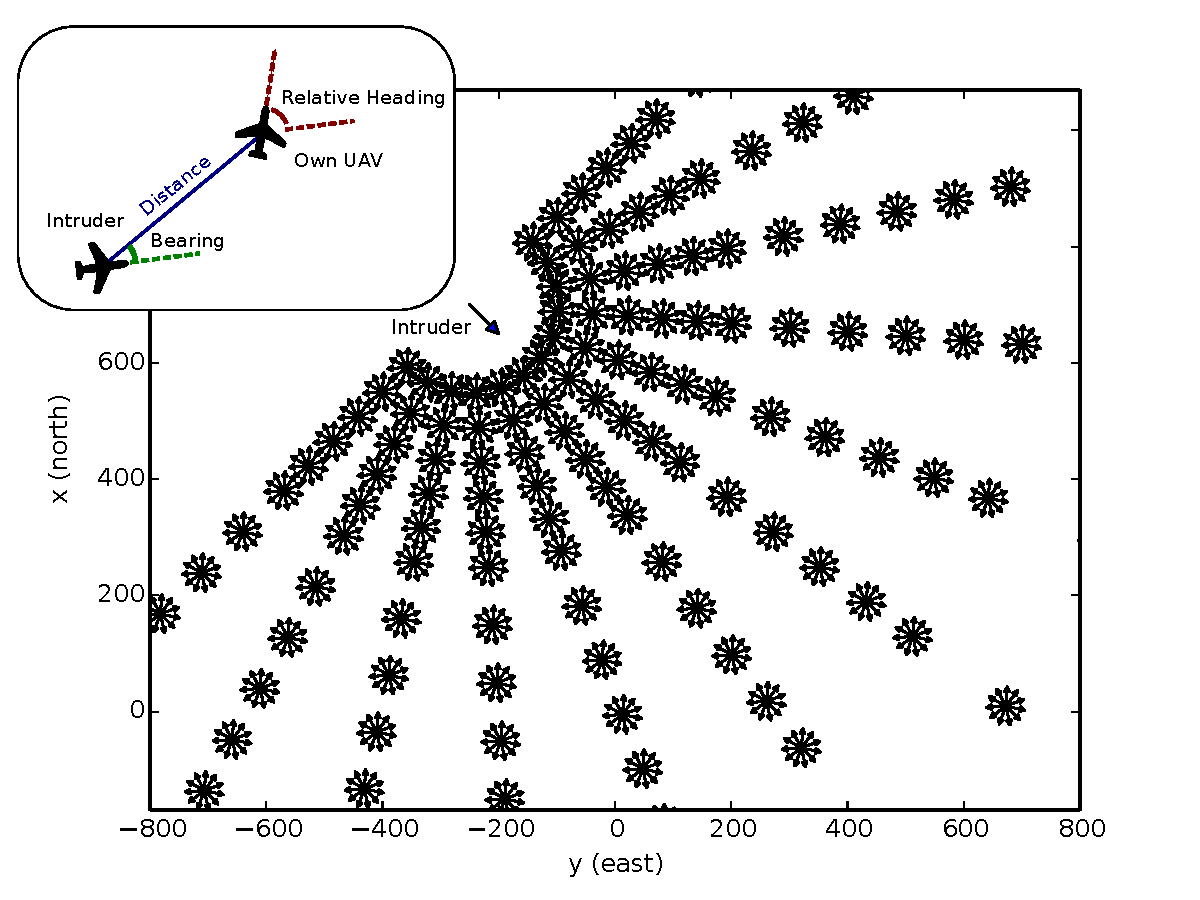
\includegraphics[width=\textwidth]{media/intruder_grid_plus.pdf}
        \caption[Intruder interpolation grid]{Intruder interpolation grid for $\beta_\text{intruder}$, visualized when the intruder is located at (\SI{700}{m}, \SI{-250}{m}) at heading \num{135}. The top left inset shows the variables used. In the main plot, each of the small arrows represents a grid point. At each of the point locations, there are twelve small arrows radiating out. Each arrow represents a different own UAV heading.}
        \label{fig:intrudergrid}
    \end{subfigure}
    \hfill
    \begin{subfigure}[t]{0.48\textwidth}
        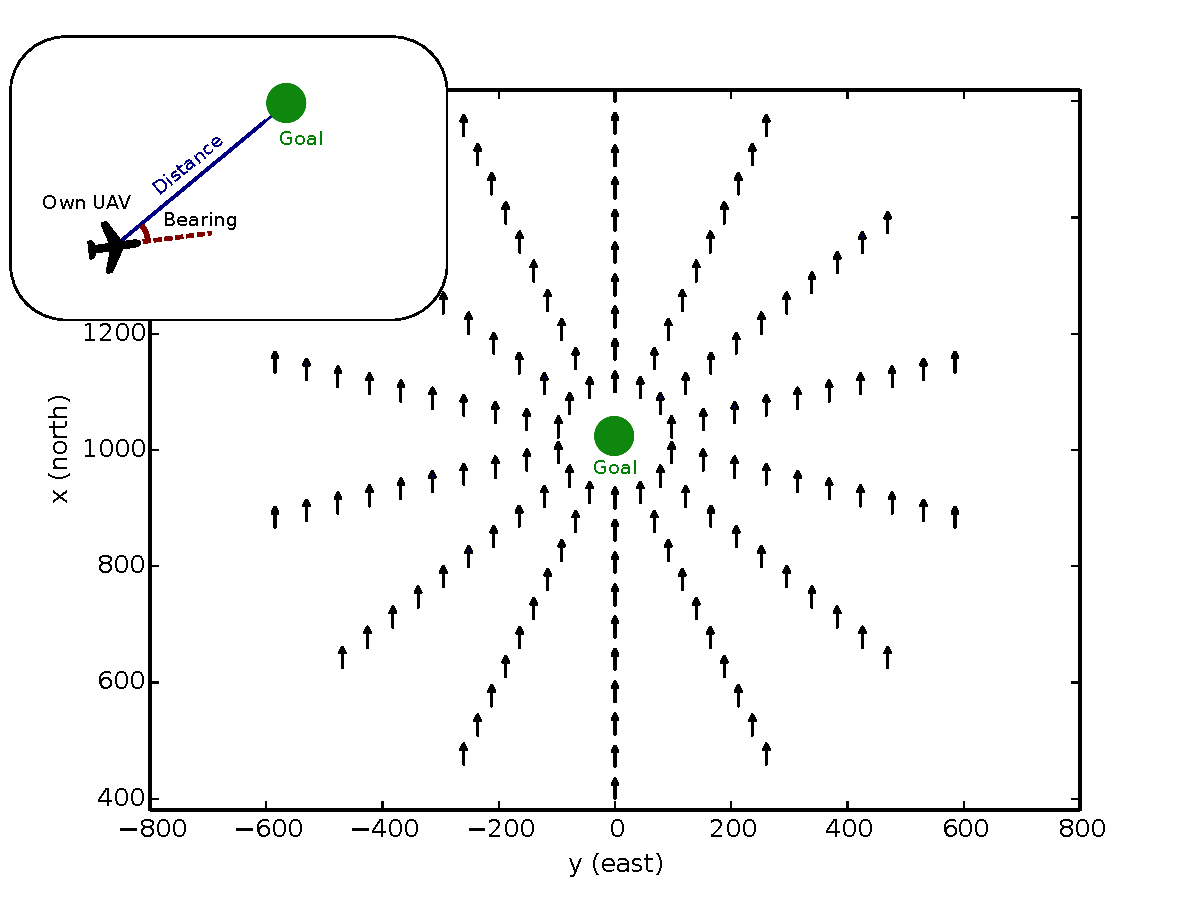
\includegraphics[width=\textwidth]{media/goal_grid_plus.pdf}
        \caption[Goal interpolation grid]{Goal interpolation grid for $\beta_\text{goal}$ when the own UAV's heading is directly north. The grid takes advantage of symmetry in the bearing variable, so, for each arrow on the left side, there is an arrow on the right side that corresponds with the \emph{same} point in the grid.}
        \label{fig:goalgrid}
    \end{subfigure}
    \caption{Value function approximation interpolation grids}
\end{figure}

Since the domain of $\beta_\text{intruder}$ is only three dimensional and the domain of $\beta_\text{goal}$ is only two dimensional, relatively fine interpolation grids can be used for value function approximation without requiring a prohibitively large number of features. The $\beta_\text{intruder}$ feature group consists of a NMAC indicator function and interpolation weights for a grid (\Cref{fig:intrudergrid}) with nodes at regularly spaced points along the following three variables: (1) the distance between the UAV and intruder, (2) the bearing from the intruder to the UAV, and (3) the relative heading between the vehicles. The $\beta_\text{goal}$ vector consists of a goal indicator function, the distance between the UAV and the goal, and interpolation weights for a grid
%(\Cref{fig:goalgrid})
with nodes regularly spaced along the distance between the UAV and the goal and the absolute value of the bearing to the goal from the UAV. The total number of features is $N_\beta = 1813$.


\section{Results} \label{sec:results}

This section presents results from numerical experiments that illustrate the effectiveness of our approach. The experiments are designed to compare the four approaches discussed in \cref{sec:uavintro}: the ``static TRL'' approach, ``direct optimization'', and the new ``optimized TRL'' and ``trusted direct optimization'' approaches proposed in this chapter. The static TRL law uses the TRL described in \cref{alg:trl} with a constant value for the separation distance (denoted with $\bar{D}$), while the other approaches use the approximate optimization procedure described in \cref{sec:approach}. The various parameters used in the numerical experiments are listed in \cref{tab:params}.

\subsection{Policies}

This section includes visualizations of two-dimensional ``slices'' of several UAV policies and their associated value functions. In each of the slices, the intruder is located at (\SI{700}{m},\SI{-250}{m}) pointed at heading 135 as indicated by the arrow. The goal is at (\SI{1000}{m},\num{0}). Each pixel on this image represents the value function or policy evaluated with the UAV at that position pointed directly north. As expected, for all approaches, there is a low value region in front of and to the south of the intruder and an increase in the value near the goal.

\Cref{fig:dovalue,fig:dopolicy} show the value function and policy for the directly optimized approach, and \cref{fig:tdovalue,fig:tdopolicy} show the same for the trusted directly optimized approach.
The policies for both approaches are similar, with regions in front of the intruder where sharp turns are commanded.
The trusted direct optimization policy is slightly more conservative with larger turn regions because of the restricted action space.

\begin{figure}[p]
    \centering
    \begin{subfigure}[t]{0.48\textwidth}
        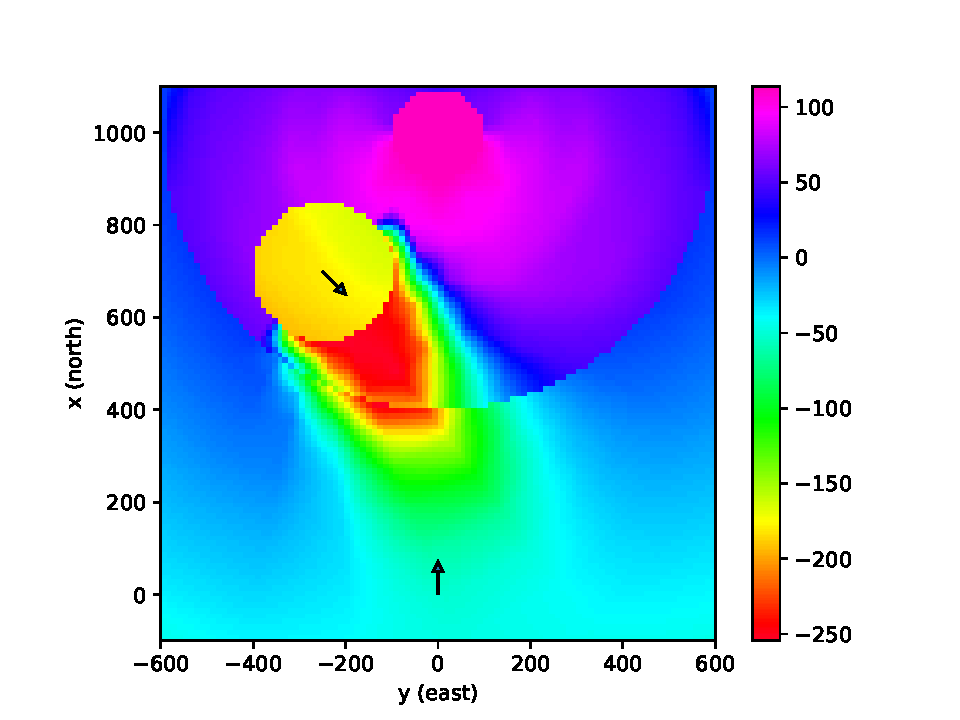
\includegraphics[width=\textwidth]{media/dovalue.pdf}
        \caption{Slice of the approximate optimal value function for direct optimization.}
        \label{fig:dovalue}
    \end{subfigure}
    \hfill
    \begin{subfigure}[t]{0.48\textwidth}
        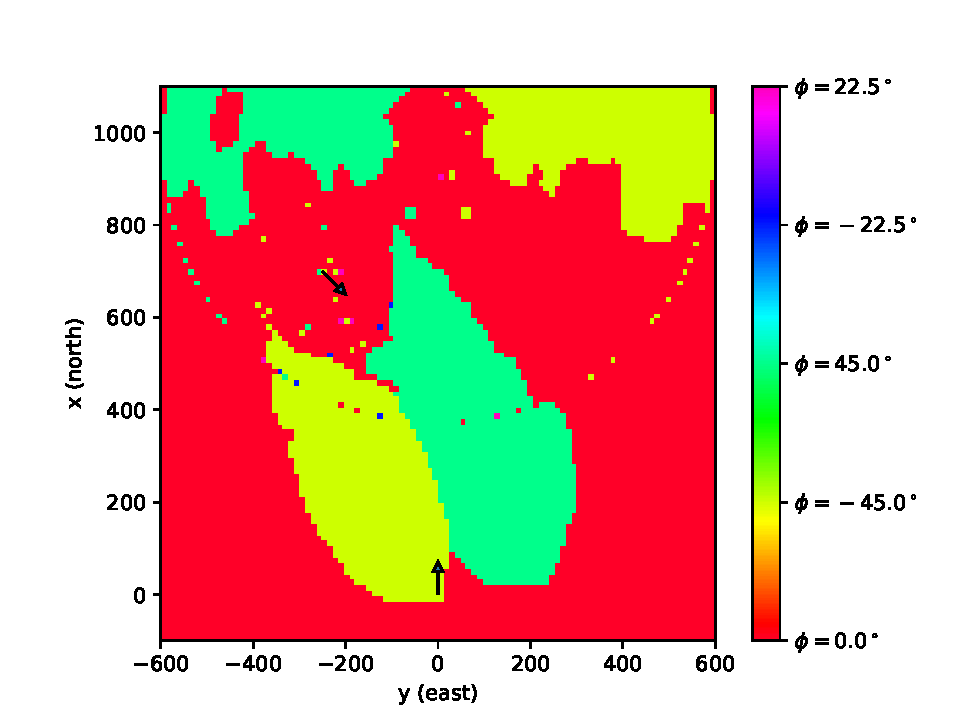
\includegraphics[width=\columnwidth]{media/dopolicy.pdf}
        \caption{Slice of the direct optimization policy.}
        \label{fig:dopolicy}
    \end{subfigure}

    \begin{subfigure}[t]{0.48\textwidth}
        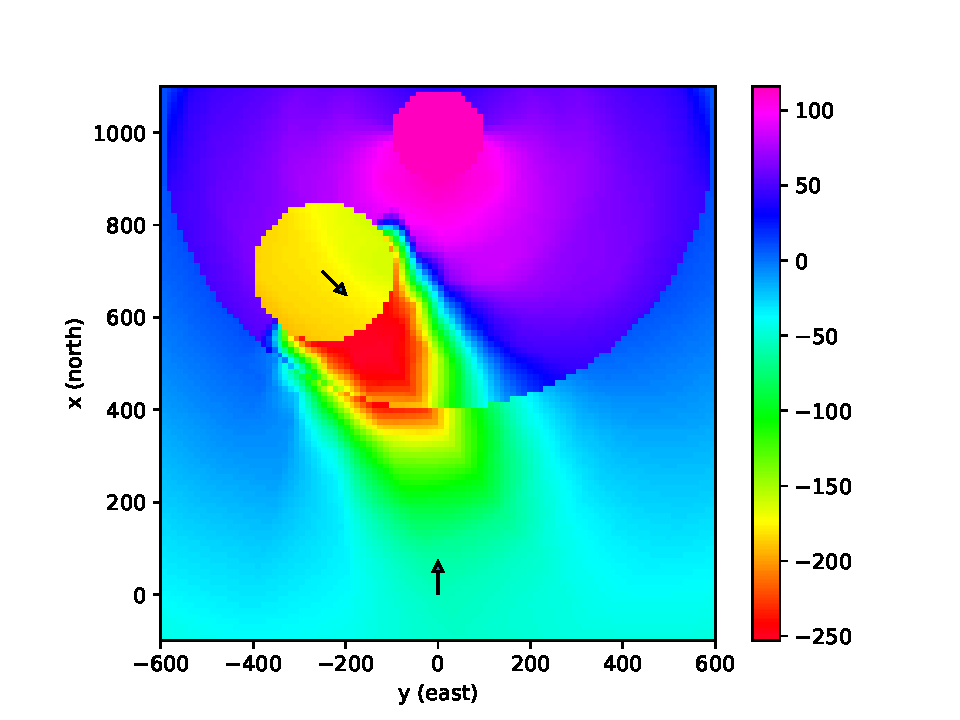
\includegraphics[width=\columnwidth]{media/tdovalue.pdf}
        \caption{Slice of the approximate optimal value function for trusted direct optimization.}
        \label{fig:tdovalue}
    \end{subfigure}
    \hfill
    \begin{subfigure}[t]{0.48\textwidth}
        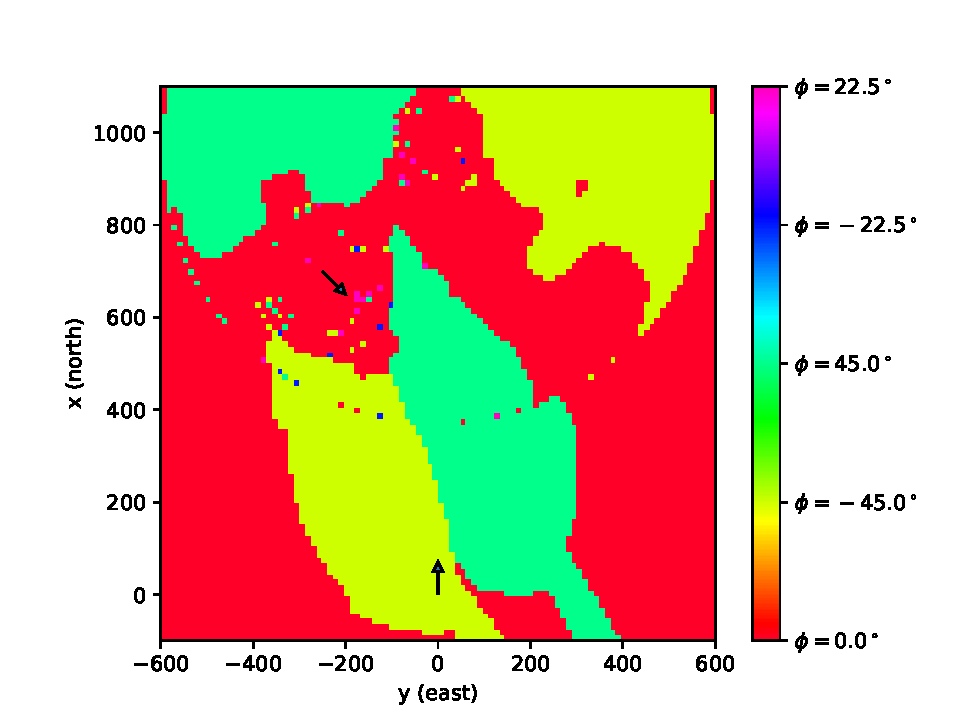
\includegraphics[width=\columnwidth]{media/tdopolicy.pdf}
        \caption{Slice of the trusted direct optimization policy.}
        \label{fig:tdopolicy}
    \end{subfigure}

    \begin{subfigure}[t]{0.48\textwidth}
        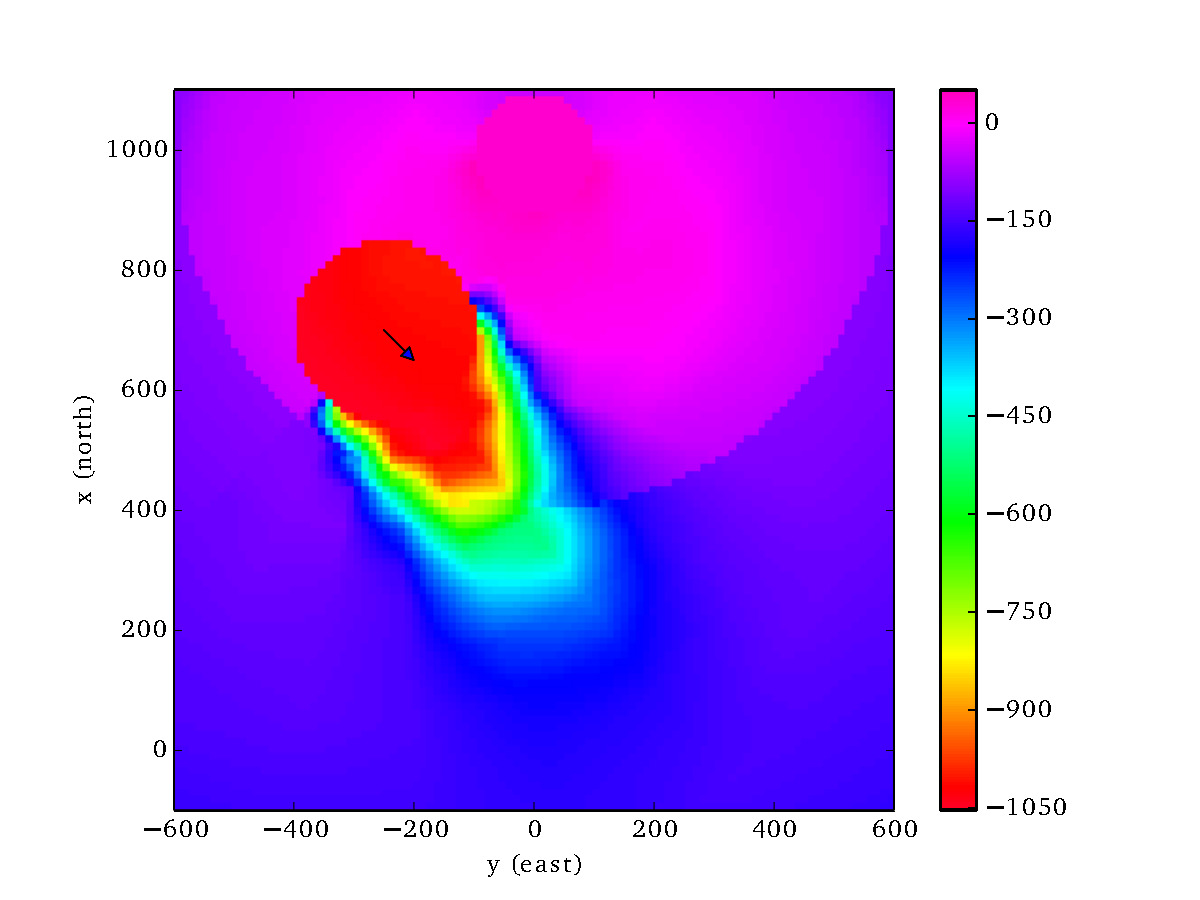
\includegraphics[width=\columnwidth]{media/value.pdf}
        \caption{Slice of the approximate optimal value function for the optimized TRL.} 
        \label{fig:trlvalue}
    \end{subfigure}
    \hfill
    \begin{subfigure}[t]{0.48\textwidth}
        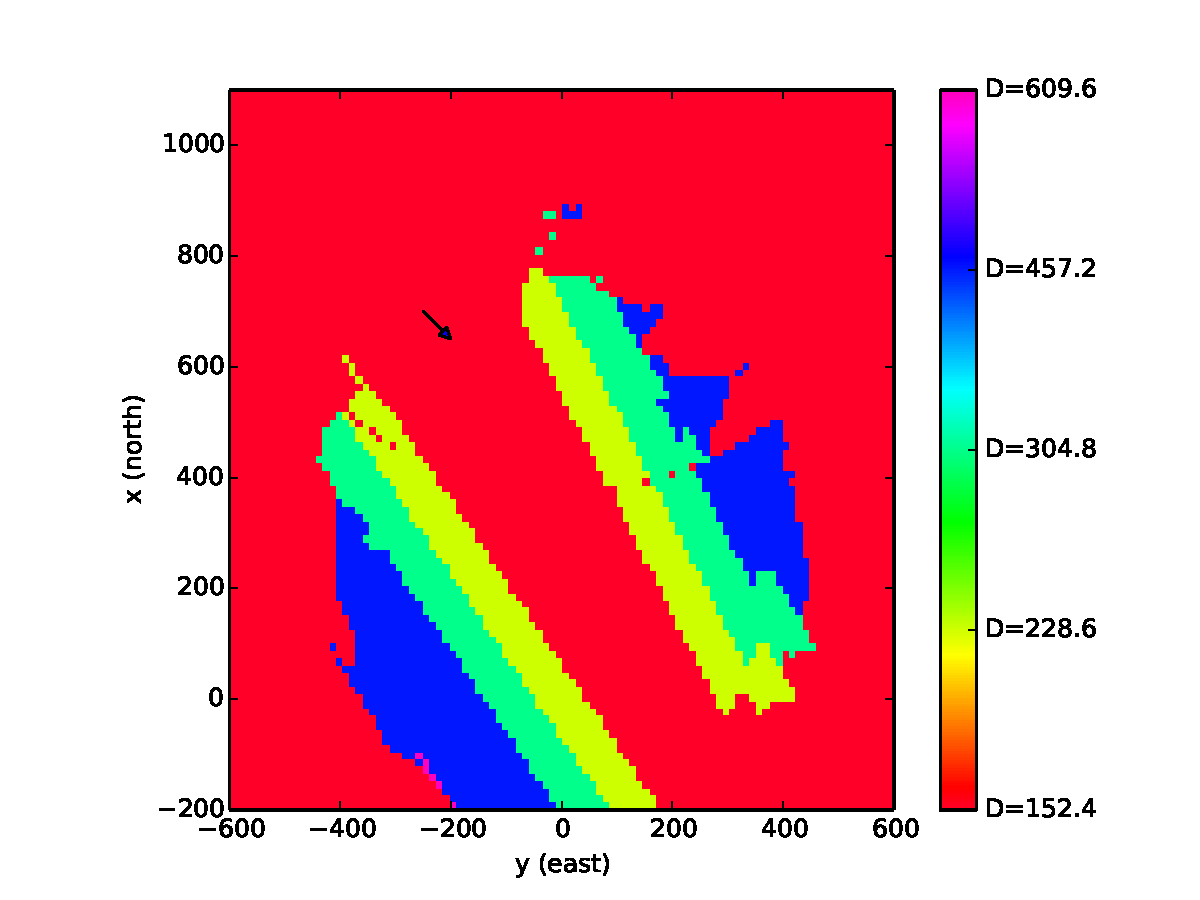
\includegraphics[width=\columnwidth]{media/policy.pdf}
        \caption{Slice of the optimized TRL policy.}
        \label{fig:trlpolicy}
    \end{subfigure}    
    \caption{UAV Collision avoidance policy visualizations}
\end{figure}



\Cref{fig:trlpolicy} shows the value function and policy for the optimized TRL approach. 
When multiple actions result in the same post decision state value, the least conservative action is chosen, so the policy yields the lowest value of $D$ ($\num{500} \si{ft} \approx \num{152.4} \si{m}$) on most of the state space. Because the own UAV is pointed north, the policy is conservative in a region in front of and to the south of the intruder. The band corresponding to small $D$ that stretches across the middle of the conservative region (from (\SI{700}{m},\SI{-250}{m}) to (\SI{-100}{m},\SI{200}{m})) is present because all values of $D$ result in the same post decision value.

\subsection{Numerical Performance Evaluation}

The control polices are evaluated by executing them in a large number of complete (from $t=0$ to the end state) encounter simulations. The same random numbers used to generate intruder noise were reused across all collision avoidance  strategies to ensure fairness of comparisons. In each of the simulations, the own UAV starts pointed north at position $(0,0)$ in a north-east coordinate system with the goal at $(1000\si{m},0)$.

The evaluation simulations use the same intruder random turn rate model with standard deviation $\sigma_{\dot{\psi}}$ that was used for value iteration. A robustness study using different models is not presented here, but previous research~\cite{MJK-JPC-PPR:10} suggests that this method will offer good performance when evaluated against both a range of noise parameters and structurally different models. The intruder initial position is randomly generated between \SI{800}{m} and \SI{1500}{m} from the center point of the encounter area at $(500\si{m},500\si{m})$ with an initial heading that is within \ang{135} of the direction from the initial position to the center point. 

The conservativeness of each control law is characterized by counting the number of deviations from the nominal path in \num{10000} simulations with initial conditions shown in \cref{fig:intruderics}.
Of these simulations, \num{1009} result in a NMAC if the UAV follows its nominal path, but for most a deviation would not be necessary to avoid the intruder.

The fraction of collisions avoided is estimated using a separate set of \num{10000} simulations. Each of these simulations has an initial condition in the same region described above, but initial conditions and noise trajectories are chosen by filtering random trials so that each of the simulations \emph{will result in a NMAC if the own UAV follows its nominal path}.

\begin{table}[tb]
    \caption{Parameters for numerical experiments} \label{tab:params}
    \centering
    \begin{tabular}{p{0.6\columnwidth} l r}
        \toprule
        Description & Symbol & Value \\
        \midrule
        Own UAV speed & $\own{v}$ & \num{30} \si{m/s} \\
        Maximum own UAV bank angle & $\phi_\text{max}$ & \ang{45} \\
        Intruder speed & $\intr{v}$ & \num{60} \si{m/s} \\
        Intruder turn rate standard deviation & $\sigma_{\dot{\psi}}$ & \ang{10}\si{/s} \\
        Near mid air collision radius & $\dnmac$ & \num{500} \si{ft} \\
        Step cost & $c_\text{step}$ & \num{1} \\
        Reward for reaching goal & $r_\text{goal}$ & \num{100} \\
        Cost for deviation & $c_\text{dev}$ & \num{100} \\
        Step simulations for expectation estimate & $N_{EV}$ & \num{20} \\
        Single step simulations per round of value iteration (optimized TRL) & $N_\text{state}$ & \num{10000} \\
        Single step simulations per round of value iteration (directly optimized) & $N_\text{state}$ & \num{50000} \\
        Number of value iteration rounds & $N_{VI}$ & \num{35} \\
        Single step simulations for post decision value function extraction & $N_q$ & \num{50000} \\
        \bottomrule
    \end{tabular}
\end{table}

\begin{figure}[tb]
    \centering
    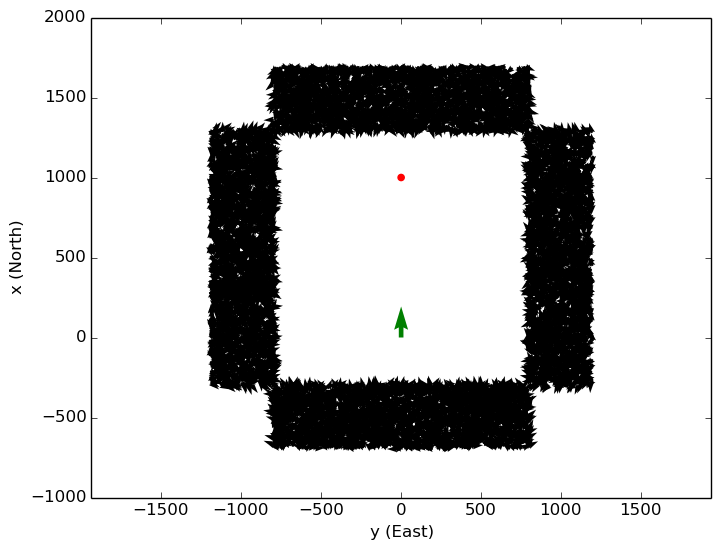
\includegraphics[width=0.8\columnwidth]{media/intruderics.png}
    \caption[Intruder initial conditions]{Intruder initial conditions for evaluation simulations. Each small black arrow is an intruder initial state. The large green arrow is the UAV's initial state. The red dot is the goal.}
    \label{fig:intruderics}
\end{figure}

\begin{figure}[tb]
    \centering
    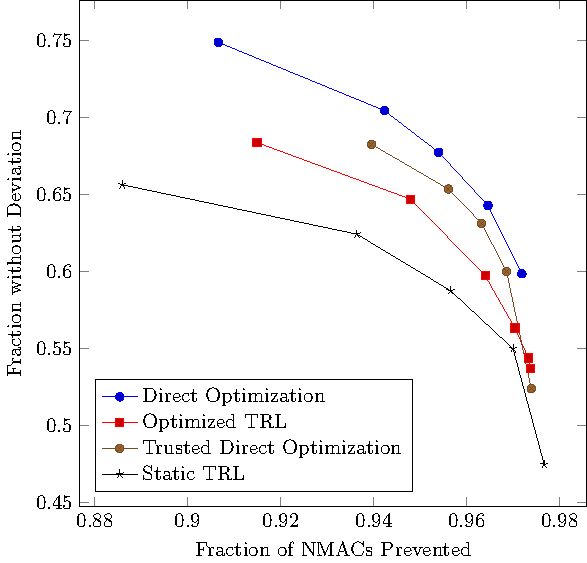
\includegraphics[width=\columnwidth]{media/pareto.pdf}
    \caption[Policy performance comparison]{Policy performance comparison. The horizontal axis variable is the number of deviations in \num{10000} encounter simulations. The values of $\lambda$ used to generate the datapoints are \num{100}, \num{316}, \num{1000}, \num{3160}, \num{e4}, and \num{3.16e4} for the optimized TRL policy and \num{300}, \num{500}, \num{700}, \num{1000}, and \num{1500} for the directly optimized approach. The values of $\bar{D}$ for the static TRL policy are \SI{250}{m}, \SI{300}{m}, \SI{350}{m}, \SI{400}{m}, and \SI{500}{m}.}
       \label{fig:pareto}
\end{figure}

\Cref{fig:pareto} shows the Pareto optimal frontiers for the different control laws. Each curve is generated by using various values of $\lambda$ in the reward function of the MDP, or by using various static values of $\bar{D}$ in the static TRL case. It is clear that the optimization provides better performance than the static TRL. For example, if the desired fraction of NMACs prevented is $96\%$, interpolation between data points suggests that direct optimization will cause approximately $20\%$ fewer deviations than the static TRL policy. This difference may be interpreted as the \emph{price} if using trusted resolution logic rather than optimization.

Fortunately, both the optimized TRL and trusted direct optimization approaches offer ways to reduce this price.
Neither should be much more difficult to certify than the TRL because they are both based on the TRL.
In particular, neither will ever command an action that is deemed unsafe by the TRL. 
Thus, they provide the same level of trust as the TRL and thus reduce the price of trust.
In this case, trusted direct optimization is able to nearly close the gap between static TRL and direct optimization, while optimized TRL reduces the gap by about half, so trusted direct optimization would be the preferred approach.


The software used to simulate these experiments was written in the Julia programming language, and is freely available at \texttt{\small{https://github.com/zsunberg/UASEncounter}}.


